\documentclass[10pt,twocolumn]{article}
\usepackage[T1]{fontenc}
\usepackage[utf8]{inputenc}
\usepackage{lmodern,microtype}
\usepackage[margin=0.73in,columnsep=0.25in]{geometry}
\usepackage{amsmath,amssymb,bm,mathtools}
\usepackage{booktabs,tabularx,array}
\usepackage{enumitem}
\usepackage{xcolor}
\usepackage{tikz}
\usetikzlibrary{arrows.meta,positioning,shapes.geometric,fit}
\usepackage{titlesec}
\usepackage{balance}
\usepackage{hyperref}
\definecolor{ink}{HTML}{17354B}
\definecolor{teal}{HTML}{117A81}
\definecolor{faint}{HTML}{EEF4F6}
\definecolor{graytext}{HTML}{536671}
\hypersetup{colorlinks=true,linkcolor=ink,urlcolor=teal,citecolor=teal,pdftitle={Speculative Sandboxes for Agentic Development: When to Fork, What to Verify, and When to Stop},pdfauthor={Yossi Eliaz}}
\setlist[itemize]{leftmargin=*,itemsep=1pt,topsep=3pt,parsep=0pt}
\setlength{\parindent}{0pt}
\setlength{\parskip}{3.25pt}
\setlength{\columnsep}{0.25in}
\setlength{\abovedisplayskip}{4pt}
\setlength{\belowdisplayskip}{4pt}
\titleformat{\section}{\large\bfseries\color{ink}}{\thesection}{0.5em}{}
\titleformat{\subsection}{\normalsize\bfseries\color{ink}}{\thesubsection}{0.5em}{}
\titlespacing*{\section}{0pt}{9pt}{4pt}
\titlespacing*{\subsection}{0pt}{7pt}{2pt}
\newcommand{\Claim}[1]{\noindent\textcolor{teal}{\textbf{#1}}\;}
\newcommand{\D}{\mathcal{D}}
\newcommand{\1}{\mathbf{1}}
\newcommand{\TV}{\operatorname{TV}}
\newcommand{\Prb}{\mathbb{P}}
\newcommand{\E}{\mathbb{E}}
\newcommand{\A}{\mathcal{A}}
\renewcommand{\arraystretch}{1.09}
\title{\vspace{-1.5em}\textcolor{ink}{\bfseries Speculative Sandboxes for Agentic Development}\\[-1pt]
\large When to Fork, What to Verify, and When to Stop}
\author{Yossi Eliaz\\[-1pt]\small Cambridge SRG seminar companion \quad\textbar\quad 13 October 2026\\[-2pt]
\small \href{https://github.com/zozo123/cam-talk-london-26}{Cambridge talk}\quad\textbar\quad
\href{https://arxiv.org/abs/2607.09689}{Evidence-aware reduction}}
\date{}
\begin{document}
\maketitle
\vspace{-1.3em}
\begin{abstract}\noindent
A speculative sandbox is an executable continuation that may be discarded. Its value is neither start-up speed nor the number of parallel agents, but verified progress relative to resource cost. We separate state fidelity, private divergence, authority and irreversible effects from the economic question of whether to fork at all. From speculative decoding we borrow draft/verify separation, adaptive depth/width and acceptance budgeting---\emph{not} exact-distribution preservation for arbitrary code. We derive correlated-success and marginal-coverage equations, distinguish verifier passes from correctness and independent evidence, and give a fail-closed controller protocol. An executable finite-world reference model tests admission, correlated replanning and receipt-bound promotion. Real sandbox integration, learned calibration and runtime gains remain \textbf{unmeasured proposals}.
\end{abstract}
\vspace{-0.5em}
\section{The framing: speculate on execution, never on authority}
A draft model proposes tokens and a target model checks them. Likewise a software controller may explore candidate changes while a separate verifier determines which exact artifact, if any, can advance. What transfers is prediction-driven allocation of speculative width, depth and checking effort. What does \emph{not} transfer is the exact decoding theorem, cheap parallel token verification or free residual correction: failed patches need diagnosis, new executions and often new tests. This is speculative execution for agentic development, not a replacement for the build cache or a new language-model decoder.

\section{First ask whether a fork should exist}

A sandbox is an \emph{execution/policy boundary}, not a synonym for a microVM or a process. A \emph{forkable continuation} is a private branch of a declared reached state $S_0$. Its contents may include filesystem, environment and optionally live memory/processes; copied guest state does \emph{not} copy the external world or publication authority. The Cambridge talk distinguishes named-snapshot \emph{restore fan-out} from live-memory fork until the nonce/process-survival probe passes \cite{cam}.

For a task class $\mathcal T$, the following are gates, not performance results:
\begin{table}[h]
\centering\footnotesize
\begin{tabularx}{\columnwidth}{@{}>{\bfseries}p{0.17\columnwidth}X@{}}
\toprule
Gate & Required evidence before claiming a useful fork\\
\midrule
State & Name the bytes, runtime state and external dependencies needed by the next action; say explicitly whether memory survives.\\
Fidelity & On pinned tasks $t\in\mathcal T$, parent and restored continuation agree on required observations under controlled seeds/inputs and declared nondeterminism; record failures.\\
Privacy & Each child gets private writes and unique runtime identity/RNG; no child can modify another's evidence or the verifier.\\
Authority & Controller owns immutable check definitions, epoch, evidence ledger and promote permission; secrets/leases are reissued, never trusted because they were copied.\\
Effects & Network/API/billing consequences are fenced, simulated, or idempotently reconciled; restore never undoes outside effects.\\
Cost & Compare against an equivalent \emph{warm cached} baseline, including capture, restore, divergence, verification and contention.\\
\bottomrule
\end{tabularx}
\caption{Operational criteria; none follows from a fast create benchmark alone.}
\end{table}

\Claim{Three distinct decisions.} \emph{Admissible} means state, privacy, authority and external-effect gates hold. \emph{Forkable} additionally requires reproducible capture/restore semantics. \emph{Advantageous} means that a fork strategy actually improves the specified utility against the best warm alternative. If any hard gate fails, do not fork; if the warm baseline wins, \emph{choose it}. Performance cannot compensate for weak isolation.

For $K$ equivalent tasks, a simple \emph{work-cost} accounting is
\begin{equation}
\label{eq:cost}
\begin{aligned}
C_{\mathrm{warm}}&=K(P_w+E+V),\\
C_{\mathrm{fork}}&=P_0+H+K(R+E+V)+D.
\end{aligned}
\end{equation}
Here $P_w$ is warm preparation, $P_0$ preparing the parent, $H$ capture, $R$ restore, $E$ execution, $V$ verification and $D$ coordination. The model assumes equivalent trials and unchanged $E,V$. Under this simplified additive model, fork saves work iff
\begin{equation}
\boxed{K P_w>P_0+H+KR+D.}
\end{equation}
For already-existing verified checkpoints, $P_0,H$ are sunk for the \emph{next} decision, but remain in complete system accounting. More generally, different execution modes can have different probabilities of success. A deadline-$T$ controller compares $U_m=B\Prb_m(\text{verified by }T)-\lambda\E_m[C]$ for $m\in\{\text{warm},\text{fork}\}$, subject to the same hard safety gates. \emph{No fork} is a first-class outcome. Tail latency and contention make wall time distinct from work cost \cite{tail}. H1 already specifies a warm-cache baseline, not a cold-start strawman \cite{cam}.

\section{What speculative decoding really proves}

Let $q(x)$ be a cheap proposal distribution and $p(x)$ the exact target distribution over tokens. Draw $x\sim q$ and accept with probability
\begin{equation}
 a(x)=\min\!\left(1,\frac{p(x)}{q(x)}\right), \qquad q(x)>0.
\end{equation}
Averaging over proposals gives \emph{maximal-coupling} acceptance:
\begin{equation}
\label{eq:tv}
\begin{aligned}
\alpha_{\rm token}
 &=\sum_x q(x)a(x)=\sum_x\min\{p(x),q(x)\}\\
 &=1-\underbrace{\frac12\sum_x|p(x)-q(x)|}_{\TV(p,q)}.
\end{aligned}
\end{equation}
Upon rejection, sample from $r(x)=[p(x)-q(x)]_+/\TV(p,q)$ when $\TV>0$. Then
\begin{equation}
\min(p,q)+\TV(p,q)r=p,
\end{equation}
pointwise. Thus the emitted token retains \emph{exactly} the target distribution; no coupling can reuse a $q$-sample with a higher probability of equality \cite{leviathan}. The theorem depends on \emph{known} $p,q$ and this correction rule.

\Claim{Never substitute a test pass for Eq.~\eqref{eq:tv}.} For code, $A_i=\{\text{exact candidate }i\text{ passes trusted checks}\}$ and $a_i=\Prb(A_i\mid\text{history})$ predicts \emph{verifier acceptance}. In general,
\begin{equation}
 1-\TV(p,q)\ne \Prb(A_i)\ne\Prb(\text{semantically correct}_i).
\end{equation}
An external verifier can still miss a bug; agent approval is not correctness. In particular, if $s=\Prb(A\mid C)$ is test sensitivity, $f=\Prb(A\mid C^c)$ is the false-pass rate, and $\pi=\Prb(C)$ is prior correctness, then
\begin{equation}
\Prb(C\mid A)=\frac{s\pi}{s\pi+f(1-\pi)},
\end{equation}
when the denominator is positive. Passing a test warrants only the claims its coverage supports. The child never controls the checker.

\subsection{A precise, but narrow, Gaussian bridge}
For two normalized Gaussians $p=N(\mu_1,\Sigma)$ and $q=N(\mu_2,\Sigma)$ with the \emph{same} positive definite covariance, the paper's two-factor weighted disagreement is
\begin{equation}
\label{eq:delta}
\Delta=\tfrac12(\mu_1-\mu_2)^T\Sigma^{-1}(\mu_1-\mu_2).
\end{equation}
Their TV overlap and KL divergence obey
\begin{equation}
\label{eq:gauss}
\boxed{\alpha_{\rm token}=2\Phi\!\left(-\sqrt{\Delta/2}\right),\quad
 D_{\rm KL}(p\|q)=\Delta.}
\end{equation}
This identity requires \emph{normalized, equal-covariance} Gaussian densities. It derives from the likelihood-ratio separating hyperplane and one-dimensional Gaussian tails. It is \emph{not} a general mapping from the reducer's disagreement to patch correctness: equal means with unequal covariances yield $\Delta=0$ but TV$>0$; identical wrong patches can agree perfectly without adding evidence \cite{eliazbmr}. The Gaussian product integral in the earlier paper is not this overlap integral.

\section{Acceptance-aware fork selection}

Let $A_i$ denote verifier acceptance and $H$ encode fork ancestors, model/prompt/test hashes, failures and known shared inputs. In a fixed trial order, define
\begin{equation}
 a_i^- =\Prb(A_i\mid H, A_1^c,\ldots,A_{i-1}^c).
\end{equation}
The chain rule gives an \emph{exact} correlated-success identity:
\begin{equation}
\label{eq:chain}
\boxed{\Prb\!\left(\bigcup_{i=1}^K A_i\middle|H\right)
=1-\prod_{i=1}^{K}(1-a_i^-).}
\end{equation}
Replacing $a_i^-$ by unconditional pass rates silently assumes independence. The history must retain observed failures and shared ancestry. Cancellation or timeout is \emph{not} a verified failure and must not be substituted for $A_i^c$ in this identity.

For a fixed set $S$ of candidate branches let $F(S)=\Prb(\bigcup_{i\in S}A_i)$. A new worker $j$ contributes
\begin{equation}
\label{eq:marginal}
\boxed{F(S\cup\{j\})-F(S)
=\Prb\!\left(A_j\cap\!\bigcap_{i\in S}A_i^c\right).}
\end{equation}
\Claim{Diversity is an objective, not decoration.} What matters is the probability that $j$ succeeds \emph{when the current workers fail}. Since the event on the right shrinks as $S$ grows, $F$ is monotone and submodular for a \emph{fixed} joint distribution. Static equal-cost greedy selection has the classic $(1-1/e)$ approximation to optimal \emph{fixed-budget coverage} \cite{nemhauser}. The guarantee does \emph{not} transfer automatically to adaptive policies or weighted cost/latency objectives; adaptive submodularity requires additional conditions \cite{golovin}.

\subsection{Concrete correlation penalty}
A transparent illustration takes a shared latent difficulty $Z\sim\operatorname{Beta}(u,v)$ and conditionally IID branch outcomes $A_i\mid Z\sim\operatorname{Bernoulli}(Z)$. Then
\begin{equation}
\begin{aligned}
\mu&=\frac{u}{u+v},\quad \rho=\frac1{u+v+1},\\
\Prb(\exists\text{ pass})&=1-\frac{(v)_K}{(u+v)_K}.
\end{aligned}
\end{equation}
With $(u,v)=(0.45,1.05)$ and $K=8$, each branch has marginal pass rate $0.30$ and pairwise outcome correlation $0.40$. The eight-branch success probability is \emph{about 65.8\%}, versus $1-0.7^8\approx94.2\%$ under independence. After four failures, the next same-family pass probability is $u/(u+v+4)=8.18\%$. These are \textbf{model calculations}, not measurements of islo or the factory.

\subsection{Depth, width, and verification cost}
For a dependent chain of $D$ speculative edits, let $L$ be the number of consecutive edits whose exact resulting artifacts pass, stopping at the first failure. The tail-sum formula is
\begin{equation}
\label{eq:prefix}
\E[L]=\sum_{j=1}^D \Prb(A_1\cap\cdots\cap A_j).
\end{equation}
If conditional prefix survival is constant $a$, then $\E[L]=\sum_{j=1}^D a^j$. Unlike token decoding, a rejected code patch has no free residual-correction token: repair, rollback, rerun and verifier invocations all cost resources.

A controller can choose depth $D$, width $W$, model/prompt diversity, verifier order and cancellation policy to maximize a budgeted objective such as
\begin{equation}
\label{eq:objective}
\max_{\pi}\;\Prb_{\pi}(\text{verified success by }T)
 -\lambda\E_{\pi}[C],
\end{equation}
subject to \emph{unrelaxed} authority and final-artifact checks. Predictive acceptance must be calibrated on held-out tasks, with latency and resource use reported jointly. EAGLE-2 and OPT-Tree motivate context-dependent tree structure; EAGLE-3 improves the proposal mechanism itself. These are inspirations, not correctness theorems for software agents \cite{eagle2,eagle3,opttree}.

\section{A runtime policy: admit, speculate, replan, stop}
\Claim{Static versus adaptive.} Fixed-set $F(S)$ is submodular; after observed failures, a sequential controller estimates
\begin{equation}
 p_j(h)=\Prb(A_j\mid h),
\end{equation}
where $h$ includes the immutable work order and completed outcomes. A simple \emph{one-step heuristic} is
\begin{equation}
 G_j(h)=B\,p_j(h)-\lambda c_j(h)-\eta\ell_j(h),
\end{equation}
with incremental total compute/verification cost $c_j$ and latency impact $\ell_j$. If no admissible $G_j>0$, stop or use warm execution. This is neither a globally optimal stopping theorem nor a production calibration model; portfolio-level parallel choices require conditional \emph{marginal} value, not sum of standalone scores.

\Claim{Which failures matter.} Distinguish \texttt{planned}, \texttt{started}, \texttt{passed}, \texttt{failed}, \texttt{timed out}, and \texttt{cancelled}. Only a trustworthy observed failure updates the \emph{success-conditioned-on-failure} probability in Eq.~\eqref{eq:chain}; absence of an outcome is censored information. When sibling failures reveal common causes, try a different hypothesis/model/fixture instead of paying for indistinguishable clones. Test the prediction on held-out workloads, not on duplicated forks of the same task.

\Claim{Issue-time effects.} A speculative API call can disclose data or incur a charge \emph{before} the branch is selected; rollback cannot unsend it. This is the ghost-tool-call issue \cite{ghost}. Fence or synthesize observable tool calls before dispatch. Separately, Sherlock studies overlap of downstream agent work with verification and rollback, but its reported benefits are not forkable-sandbox measurements \cite{sherlock}.

\section{Acceptance is not independent evidence}

In the paper's independent Gaussian common-target model, worker $i$ returns estimate $\hat\theta_i$, information $P_i$, evidence IDs and lineage. The current reducer forms $P=\sum_iP_i$ and $q=\sum_i P_i\hat\theta_i$, rejects declared duplicate IDs and transports ancestry. It \emph{does not} infer covariance from lineage or implement selection correction \cite{eliazbmr}.

If estimates share latent error $U$ and have independent noise $\varepsilon_i$, write $Y_i=\theta+U+\varepsilon_i$ with variances $\tau^2$ and $\sigma^2$. Then
\begin{equation}
\operatorname{Var}(\bar Y)=\tau^2+\frac{\sigma^2}{K},\quad
K_{\rm eff}=\frac{K}{1+(K-1)\rho},
\end{equation}
where $\rho=\tau^2/(\tau^2+\sigma^2)$. Eight estimates with $\rho=0.4$ have $K_{\rm eff}\approx2.11$ under this model. \emph{Acceptance correlation} and \emph{estimation-error correlation} are separate quantities; this effective sample size is not a success-probability shortcut.

With a \emph{justified} covariance matrix $C$ and a common-target observation map $H_0$, generalized least squares gives
\begin{equation}
\label{eq:gls}
\begin{aligned}
\hat\theta&=(H_0^TC^{-1}H_0)^{-1}H_0^TC^{-1}Y,\\
\operatorname{Cov}(\hat\theta)&=(H_0^TC^{-1}H_0)^{-1}.
\end{aligned}
\end{equation}
A candidate fork-DAG covariance model is $C_{ij}=\sum_{a\in\mathrm{Anc}(i)\cap\mathrm{Anc}(j)}T_a+\1_{i=j}R_i$. Ancestry alone does \emph{not} identify these variance components: fit/validate them externally or \textbf{abstain} from claiming increased precision.

\Claim{Selection creates another bias.} Suppose 100 IID $N(\theta,1)$ estimates each report $[Y_i-1.96,Y_i+1.96]$. If we choose the largest estimate, coverage becomes
\begin{equation}
\Prb(\theta\in I_{\arg\max Y_i})
=\Phi(1.96)^{100}-\Phi(-1.96)^{100}\approx 7.95\%.
\end{equation}
So even initially valid 95\% intervals may become invalid after choosing winners. A valid reducer must record \emph{rejections and selection history}, then use simultaneous/selection-aware or held-out inference; unchanged marginal intervals are not automatically valid after search. This is a \textbf{synthetic calculation}, not measured agent behavior.

\section{A minimal end-to-end controller}
\begin{figure}[h]
\centering
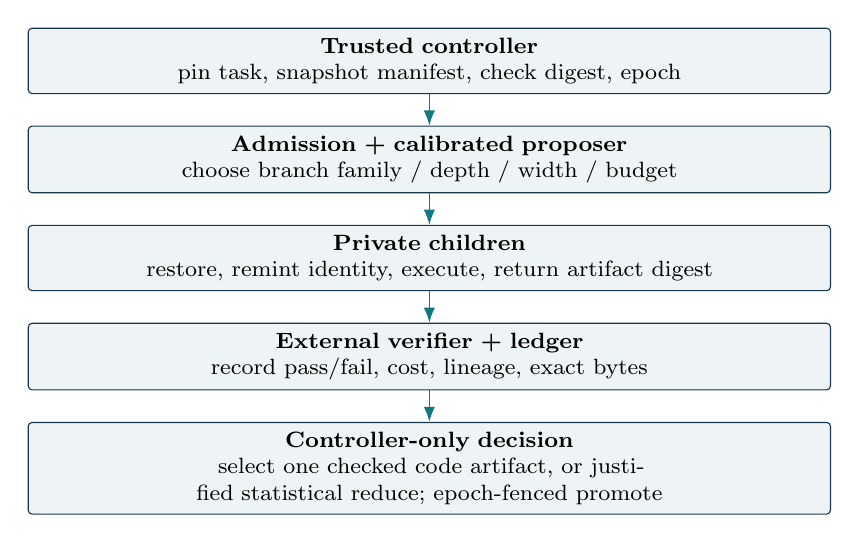
\begin{tikzpicture}[node distance=4mm,>=Latex,
 box/.style={draw=ink,rounded corners=1.4pt,fill=faint,align=center,inner sep=3.5pt,text width=0.82\columnwidth,font=\footnotesize},
 flow/.style={->,line width=0.55pt,draw=teal}]
\node[box] (root) {\textbf{Trusted controller}\\pin task, snapshot manifest, check digest, epoch};
\node[box,below=of root] (fork) {\textbf{Admission + calibrated proposer}\\choose branch family / depth / width / budget};
\node[box,below=of fork] (run) {\textbf{Private children}\\restore, remint identity, execute, return artifact digest};
\node[box,below=of run] (check) {\textbf{External verifier + ledger}\\record pass/fail, cost, lineage, exact bytes};
\node[box,below=of check] (prom) {\textbf{Controller-only decision}\\select one checked code artifact, or justified statistical reduce; epoch-fenced promote};
\draw[flow] (root)--(fork);\draw[flow](fork)--(run);\draw[flow](run)--(check);\draw[flow](check)--(prom);
\end{tikzpicture}
\caption{Proposed protocol. Only the controller can issue the final promote operation.}
\end{figure}

\Claim{Admission.} An immutable work-order key binds repository tree, initial-state digest, tool/model/prompt versions, task and selection context. Retried evaluation of \emph{the same observation} reuses its evidence token; new samples get new tokens, but keep common ancestry. Do not count retries or speculative replicas twice.

\Claim{Execution.} Keep warm compiler/dependency state where safe, while child writes remain private; reseed uniqueness and remint authority outside copied guest state. Cheap tests may reject drafts early but cannot replace the sealed final verifier. Cancel losers only after their outcome/selection-accounting obligations are satisfied; mark cancelled outcomes \emph{unobserved}, not failed.

\Claim{Verification.} An external checker binds \texttt{(task/input, artifact bytes, verifier digest, evaluation ID, epoch, verdict)} to a controller-authenticated receipt. Persist both passes and negative/censored outcomes. A \emph{green} receipt asserts the specified checks ran on these bytes; it does not prove general program correctness. Different result types have different fan-in: select one patch, recheck any composed patch, or pool common-target measurements only with justified covariance.

\Claim{Publication.} Persist exact artifact bytes and checks before teardown; compare current epoch/version at a single controller-owned compare-and-swap. Stale workers can finish but cannot publish. Untrusted children must never write scores, sealed tests, receipts or promote tokens. The seminar's serial factory records motivate these obligations but do not demonstrate the complete forked protocol \cite{cam}.

\section{Executable toy and mathematical audit}
An executable finite-world simulator and two standard-library test suites accompany this note. The \emph{finite-world model} defines explicit, hypothetical joint pass events; its probabilities are known by construction, \emph{not fitted} from real agents. It demonstrates all-or-nothing admission gates, a warm-cache win, a perfect-duplicate sibling worth no extra coverage, posterior replanning after verified failures, stopping when expected value is negative, and distinct timeout/cancellation semantics.

The \emph{controller mock} persists candidate bytes, executes an externally held predicate and authenticates a digest/epoch/evaluation-ID receipt before one promotion. Tests deliberately try altered artifacts, altered receipts, repeated evaluation tokens, stale epochs and an \emph{incomplete checker that passes bad code}. The last case makes the distinction between a validated protocol and semantic correctness explicit. HMAC, in-memory persistence and the finite-world oracle are demonstration choices; no isolation, robust key service, durable atomic transaction or actual microVM is implemented.\par
Independent checks recompute TV residual mass, Gaussian overlap by numerical quadrature, conditional chain probabilities, submodularity, beta-binomial success, expected accepted-prefix length, generalized least squares, post-selection coverage and the cost identity.

\section{Falsifiable evaluation, not a speedup claim}

\textbf{Preserve preregistration.} The Cambridge \texttt{PREREGISTRATION.md} already fixes Gate~0 (memory nonce), fidelity, H1 warm-cache cost and H2 sibling-vs-stranger correlation, with predefined tests and rejection thresholds. Do \emph{not} change those analyses or imply they have run. The following is a separately labelled \textbf{exploratory Phase D proposal}.

\begin{enumerate}[leftmargin=*,itemsep=1pt,topsep=2pt]
\item \textbf{Same tasks, same authority:} pin repositories, work orders, checker images/digests, snapshot semantics and compute/time budgets; compare serial warm, fixed-width fan-out, calibrated acceptance-only, and lineage-aware adaptive scheduling.
\item \textbf{Predict before seeing the outcome:} train conditional pass models on disjoint historical tasks; freeze and calibrate them; record predictive log loss, Brier score and reliability by fork family, failure class and workload difficulty.
\item \textbf{Measure complete cost:} prepare/capture/restore, agent calls, verifier executions, cancellation, external effects, queueing, memory and p50/p95 time-to-\emph{first exact verified artifact}; count CPU-seconds and dollars per success. Include no-fork/warm-cache controls.
\item \textbf{Try hard negative controls:} cloned wrong assumptions, independent model/prompt families, the \texttt{CellBusy} path without its direct deterministic test, stale epochs, duplicate evidence, tampered oracle, speculative observable API calls and post-selection intervals.
\item \textbf{Report falsifiers:} adaptive speculation must beat the best \emph{warm} mode on cost/verified-progress or deadline performance; lineage complexity is warranted only by better held-out conditional predictions or defensible coverage. Report null, worse, timeout and verifier false-pass outcomes, not only winning attempts.
\end{enumerate}

\textbf{Talk placement.} A 90-second optional Q\&A bridge after the seminar's runtime/evidence boundary: \emph{``A fork is worthwhile only if it preserves useful state, beats the warm alternative on verified progress per budget, and cannot grade or publish itself. Speculation then asks: what is the probability this \emph{next} branch succeeds \emph{when the existing branches fail}? That probability controls the scheduler, while independent evidence controls statistical confidence.''}

\section*{Takeaway}
\noindent\colorbox{faint}{\parbox{0.94\columnwidth}{\vspace{4pt}\small\textbf{Fork only when admissible and better than the warm alternative.\newline
Speculate on candidates; externally verify exact bytes; replan after negative evidence; promote once. Count statistical confidence by provenance and calibrated dependence, never by green-check or worker counts.}\vspace{4pt}}}

\balance
\begin{thebibliography}{13}\footnotesize\setlength{\itemsep}{1pt}
\bibitem{cam} Y. Eliaz, \href{https://github.com/zozo123/cam-talk-london-26}{\emph{Forkable Sandboxes Cambridge Seminar}}, 2026. Claim fence and preregistration in the repository.
\bibitem{eliazbmr} Y. Eliaz, \href{https://arxiv.org/abs/2607.09689}{\emph{Evidence-Aware Reduction for Forkable Compute}}, arXiv:2607.09689v4, 2026.
\bibitem{leviathan} Y. Leviathan, M. Kalman, Y. Matias, \href{https://proceedings.mlr.press/v202/leviathan23a.html}{\emph{Fast Inference from Transformers via Speculative Decoding}}, ICML, 2023.
\bibitem{eagle2} Y. Li et al., \href{https://aclanthology.org/2024.emnlp-main.422/}{\emph{EAGLE-2: Faster Inference of Language Models with Dynamic Draft Trees}}, EMNLP, 2024.
\bibitem{eagle3} Y. Li et al., \href{https://papers.neurips.cc/paper_files/paper/2025/hash/c7b5a35ea98b62512a869c19ea7b03cb-Abstract-Conference.html}{\emph{EAGLE-3: Scaling up Inference Acceleration of Large Language Models via Training-Time Test}}, NeurIPS, 2025.
\bibitem{nemhauser} G. L. Nemhauser, L. A. Wolsey, M. L. Fisher, \emph{An Analysis of Approximations for Maximizing Submodular Set Functions---I}, Mathematical Programming 14, 1978.
\bibitem{golovin} D. Golovin, A. Krause, \href{https://arxiv.org/abs/1003.3967}{\emph{Adaptive Submodularity: Theory and Applications in Active Learning and Stochastic Optimization}}, JAIR, 2011.
\bibitem{opttree} J. Wang et al., \href{https://aclanthology.org/2025.tacl-1.8/}{\emph{OPT-Tree: Speculative Decoding with Adaptive Draft Tree Structure}}, TACL 13, 2025.
\bibitem{ghost} B. Mohammadi et al., \href{https://arxiv.org/abs/2606.02483}{\emph{Ghost Tool Calls: Issue-Time Privacy for Speculative Agent Tools}}, arXiv:2606.02483, 2026.
\bibitem{sherlock} Y. Ro et al., \href{https://www.microsoft.com/en-us/research/publication/sherlock-reliable-and-efficient-workflow-execution/}{\emph{Sherlock: Reliable and Efficient Workflow Execution}}, 2025.
\bibitem{tail} J. Dean, L. A. Barroso, \href{https://research.google/pubs/the-tail-at-scale/}{\emph{The Tail at Scale}}, CACM 56(2), 2013.
\end{thebibliography}
\end{document}